% In \autoref{sec:circuitelement}, we discussed that at high frequency, lumped circuit elements such as the inductor do not behave only as an inductor, but as a capacitor and an inductor. Also, a capacitor does not behave only as a capacitor, but as an inductor and a capacitor. Due to this behaviour experienced by these lumped elements (capacitor and inductor) at high frequencies, a transmission line of length $l$ with a short circuit or open circuit end is used.

% A short circuited transmission line has a length, $l_{SC}$ and a open circuited transmission line has a length $l_{OC}$. it is used as a capacitor and as an inductor by varying its length. We established that for an inductor, $0 < l_{SC} < \frac{\lambda}{4}$ and for a capacitor, $\frac{\lambda}{4} < l_{SC} < \frac{\lambda}{2} $

% Up to this point, we have dealt with a lossless transmission line, which implies, for the use of the transmission line as a resonant circuit, we expect to get an infinite quality factor. Quality factor\index{quality factor} of a resonance circuit depends on the losses of the circuit, higher loss leads to low-quality factor and vice versa.

Let us consider a transmission line with losses at the length of $ l=\frac{\lambda}{4}$ so that we can then determine the actual value of the quality factor for this case. The transmission line can be either an open circuit or a short circuit as shown in figure~\ref{fig:fig1}.
\begin{figure}[h]
\centering
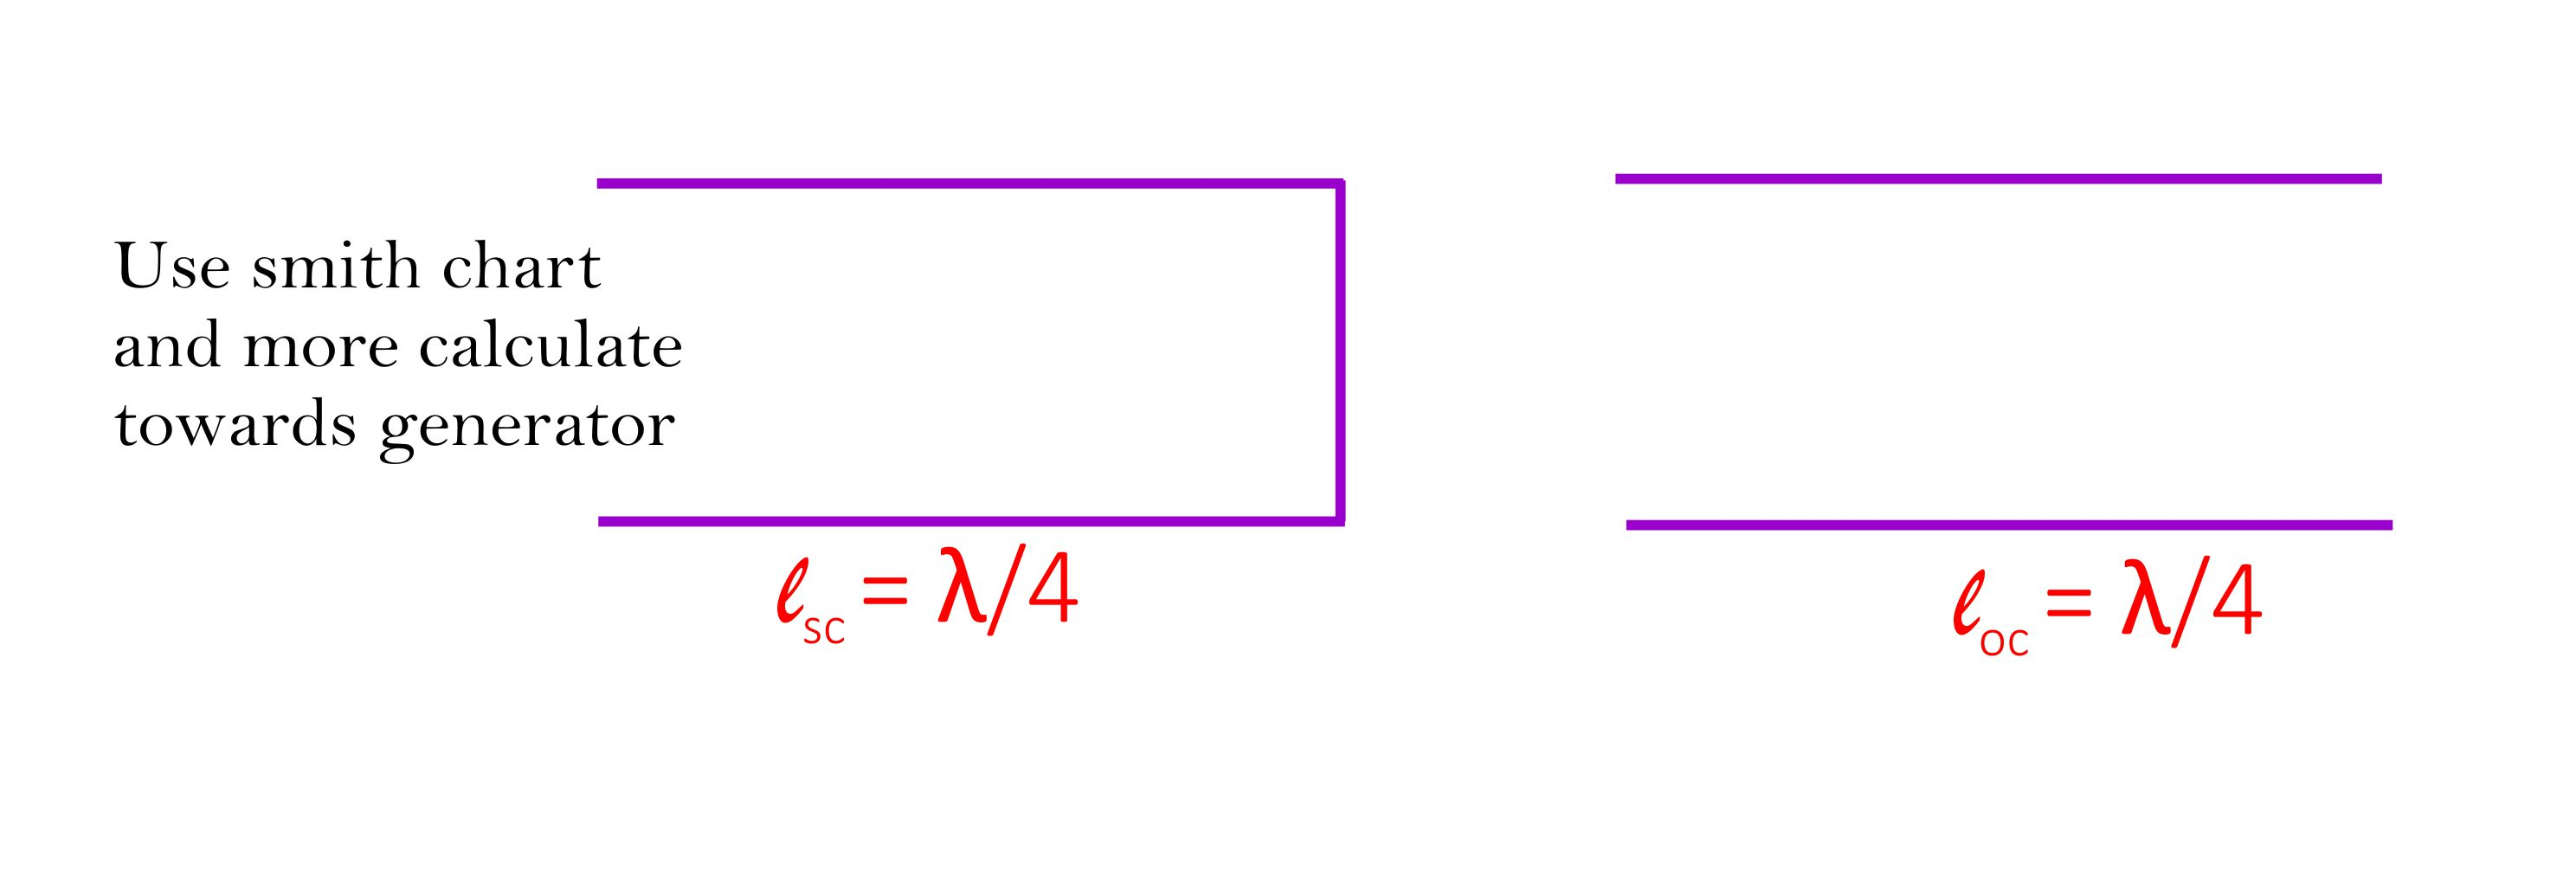
\includegraphics[width=1\linewidth]{\pathtopartone/graphics/fig1}
\caption{Short and Open Circuit end transmission line of length $\frac{\lambda}{4}$}
\label{fig:fig1}
\end{figure}

At $ \frac{\lambda}{4} $, the open circuit will appear as a short circuit to the other end of the line and similarly, the short circuit will appear as an open circuit. Therefore, a short circuit end transmission line will appear as a parallel resonance circuit at $ l_{SC}=\frac{\lambda}{4} $ and an open circuit end transmission line will appear as a series resonance circuit at $ l_{OC}=\frac{\lambda}{4} $. So, in order to find the quality factor, we first calculate the actual input impedance of these lines with losses at the given length.

\subsubsection{Impedance of resonant circuit with losses}\label{lec:lec11}
To calculate the input impedances of the lines $ Z_{OC} $ and $ Z_{SC} $, for a length $ l=\frac{\lambda}{4} $ with losses, recall the impedance transformation relationship is
\begin{dmath*}
Z(l) = Z_0\left(\frac{Z_{L}\cosh\gamma l + Z_0\sinh\gamma l}{Z_0\cosh\gamma l + Z_{L}\sinh\gamma l}\right)\quad\text{for short circuit }Z_{L}\text{= 0}
= Z_0\left( \frac{0\times\cosh\gamma l + Z_0\sinh\gamma l}{Z_0\cosh\gamma l + 0\times\sinh\gamma l}\right)
= Z_0\left(\frac{Z_0\sinh\gamma l}{Z_0\cosh\gamma l}\right)
= Z_0\left(\frac{\sinh\gamma l}{\cosh\gamma l}\right)
\end{dmath*}
From trigonometry functions $ \tanh\theta =\frac{\sinh\theta}{\cosh\theta} $
\begin{equation}
Z(l)_{SC}=Z_0\tanh\gamma L
\end{equation}
We adjust the expression for open circuit length at $ Z_{L} =\infty $ and take limits at it tends to $\infty$, thus
\begin{dmath*}
Z(l)_{OC} = Z_0\left(\frac{\cosh\gamma l +\frac{Z_0}{Z_{L}}\sinh\gamma l}{\frac{Z_0}{Z_{L}}\cosh\gamma l+ \sinh\gamma l}\right)
= Z_0\left(\frac{\cosh\gamma l + 0\times\sinh\gamma l}{0\times\cosh\gamma l+ \sinh\gamma l}\right)
= Z_0\left(\frac{\cosh\gamma l}{\sinh\gamma l}\right)
\end{dmath*}
From trigonometry functions $ \frac{1}{\tanh\theta}=\frac{\cosh\theta}{\sinh\theta}=\coth\theta $
\begin{equation}
Z(l)_{OC}=Z_0\coth\gamma l	
\end{equation}
$ Z(l)_{SC}=Z_0\tanh\gamma l $ and $ Z(l)_{OC}=Z_0\coth\gamma l $, but with $ \gamma=\alpha +j\beta $, we have $ \alpha\ll\beta $ for low loss transmission line\footnote{
A low-loss transmission line is not the same as a lossless transmission line
}, i.e $ \gamma\neq j\beta $, the $ \alpha $ part must be taken into consideration as well. We know that at $ l=\frac{\lambda}{4} $, the input impedance of a short circuit line is an open circuit and that of an open circuit line is a short circuit. However, in the presence of a loss, that will not be true. The impedance will neither be infinity for $ Z_{SC} $ nor zero for $ Z_{OC} $. If the loss is present, the input impedance will give
\begin{equation}
Z_{SC}=Z_0\tanh\gamma l=Z_0\tanh(\alpha+j\beta)l
\end{equation}
Where $ \gamma=\alpha+j\beta $ for a low-loss transmission line.

From trigonometry $\tanh(A+B)=\frac{\tanh A+\tanh B}{1+\tanh A\tanh B} $
\begin{equation}
\tanh(\alpha+j\beta)l=\frac{\tanh (\alpha l) + \tanh (j\beta l)}{1 + \tanh (\alpha l)\tanh (j\beta l)}
\end{equation}
Recall that $ \tanh jA= j\tan A$.\\
Therefore,
\begin{equation}
Z_0\tanh(\alpha+j\beta)l=Z_0\left(\frac{\tanh \alpha l+j\tan \beta l}{1+j\tanh \alpha l\tan \beta l}\right)
\end{equation}
If $ \alpha $ is small compare to $ \beta $ for a length of $ \frac{\lambda}{4} $ of transmission line, $ \alpha l $ is much smaller than 1. For a low loss line, $ \alpha\ll\beta $ and $ \beta=\frac{2\pi}{\lambda} $. Therefore	$ \tanh \alpha l \approxeq \alpha l $, then we have
\begin{equation}
Z_{SC}\approxeq Z_0\left(\frac{\alpha l + j \tan \beta l}{1+ j\alpha l \tan\beta l}\right)
\label{eqn:scimp}
\end{equation} 
For $ l=\frac{\lambda}{4}, \beta=\frac{2\pi}{\lambda} \Longrightarrow \beta l= \frac{2\pi}{\lambda} \times\frac{\lambda}{4} =\frac{\pi}{2} $\\
Dividing both the numerator and denominator of equation~\ref{eqn:scimp} by $ \tan\beta l $
\begin{dmath*}
Z_{SC}=Z_0\left(\frac{\alpha l + j \tan \beta l}{1+ j\alpha l \tan\beta l}\right)\times\left(\frac{\frac{1}{\tan \beta l}}{\frac{1}{\tan \beta l}}\right)
=Z_0\left(\frac{\frac{\alpha l}{\tan \beta l}+\frac{j\tan \beta l}{\tan \beta l}}{\frac{1}{\tan \beta l}+\frac{j\alpha l\tan \beta l}{\tan \beta l}}\right)
=Z_0\left(\frac{\frac{\alpha l}{\tan \beta l} + j}{\frac{1}{\tan \beta l} + j\alpha l}\right)\quad \tan \beta l\text{ =}\tan\frac{\pi}{2}\text{ =}\infty 
=Z_0\left(\frac{\frac{\alpha l}{\infty} + j}{\frac{1}{\infty} + j \alpha l}\right)\quad\frac{\alpha l}{\infty}\text{= 0, }\frac{1}{\infty}\text{= 0}
=Z_0\left(\frac{j}{j\alpha l}\right)
=Z_0\left(\frac{1}{\alpha l}\right)
\end{dmath*}
\begin{equation}
Z_{SC}=\frac{Z_0}{\alpha l}
\end{equation}
Therefore, this means that the input impedance of a short circuit line, if the length is $ \frac{\lambda}{4} $ is $ \frac{Z_0}{\alpha l} $, which is not infinity. Recall $ Z_{SC} = \infty $ for a lossless transmission line, but $ \alpha l \ll 1 $ means $ Z_{SC} $ is large but not infinity.

Similarly, the open circuit impedance is 
\begin{dmath*}
Z_{OC}=Z_0\coth\gamma l=\frac{Z_0}{\tanh\gamma l}
=Z_0\coth\gamma l=Z_0\coth(\alpha+j\beta) l
\end{dmath*}
For low loss transmission line $ \alpha\ll\beta $.

Recall, 
\[ \tanh(\alpha+j\beta)l=\frac{\tanh (\alpha l) + \tanh (j\beta l)}{1 + \tanh (\alpha l)\tanh (j\beta l)} \]
But,
\[ \frac{1}{\tanh(\alpha+j\beta)l}=\frac{1 + j\tanh (\alpha l)\tanh (j\beta l)}{\tanh (\alpha l) + \tanh (j\beta l)} \]
And lastly, $ \tanh jA= j \tan A $
\begin{dmath*}
Z_{OC} = \frac{Z_0}{\tanh(\alpha+j\beta)}
=Z_0\left(\frac{1+j\tanh \alpha l\tan \beta l}{\tanh \alpha l+j\tan \beta l}\right)
\approxeq Z_0\left(\frac{1+ j \alpha l\tan \beta l}{\alpha l+j\tan \beta l}\right)
\end{dmath*}
Divide both the numerator and denominator by $ \tan \beta l $
\begin{dmath*}
Z_{OC}=Z_0\left(\frac{\frac{1}{\tan \beta l}+\frac{j \alpha l\tan \beta l}{\tan \beta l}}{\frac{\alpha l}{\tan \beta l}+\frac{j\tan \beta l}{\tan \beta l}}\right)
=Z_0\left(\frac{\frac{1}{\tan \beta l} + j \alpha l}{\frac{\alpha l}{\tan \beta l} + j}\right)\quad\tan\beta l\text{ =}\tan\frac{\pi}{2}\text{= }\infty
=Z_0\left(\frac{\frac{1}{\infty} + j \alpha l}{\frac{\alpha l}{\infty} + j}\right)\quad\frac{\alpha l}{\infty}\text{= 0, }\frac{1}{\infty}\text{= 0}
=Z_0\left(\frac{j \alpha l}{j}\right)
\end{dmath*}
\begin{equation}
Z_{OC}=Z_0(\alpha l)
\end{equation}
Therefore, for low loss transmission line where $\alpha\ll\beta$, $ Z_{SC}\approxeq \frac{Z_0}{\alpha l} $ and $ Z_{OC} \approxeq Z_0 \alpha l $. 

Ideally $ Z_{OC}=0 $, but this is not the case with the low-loss line where we have $ Z_{OC} = Z_0 \alpha l $. What we note here is that the input impedance of the resonance section of a transmission line is ideally zero or infinity for series or parallel resonance circuits respectively. In practice, we see that we have a small input impedance for a series resonance circuit and a large input impedance for a parallel resonance circuit.

With $ Z_{OC} = Z_0 \alpha l $ and 
$ Z_{SC}= \frac{Z_0}{\alpha l} $, we can vary the frequency and measure the variation of $ Z_{SC} $ or $ Z_{OC} $ with frequency. Recall that $ \alpha $ depends on frequency, length $(l)$ also depends on frequency since $ l=\frac{\lambda}{4} $. The variation of $ Z_{SC} $ or $ Z_{OC} $ with frequency gives us what is called the frequency response of the circuit\index{frequency response of the circuit}.

\subsubsection{Quality factor}
Quality factor\index{quality factor} can be calculated in two ways:
\begin{enumerate}[(i)]
\item From the frequency response of the circuit
\item From the basic definition of quality factor.
\end{enumerate}
The quality factor (Q factor) can be computed from the frequency response of a system. The Q factor is a measure of the damping in a system and is related to the sharpness of the resonance peak in the frequency response. If we plot the current or voltage response when a current or voltage source is applied to the input of the section of the transmission line and we measure the 3dB bandwidth of the response, the centre frequency divided by the 3dB bandwidth of the frequency response gives the quality factor.
\begin{figure}[h]
\centering
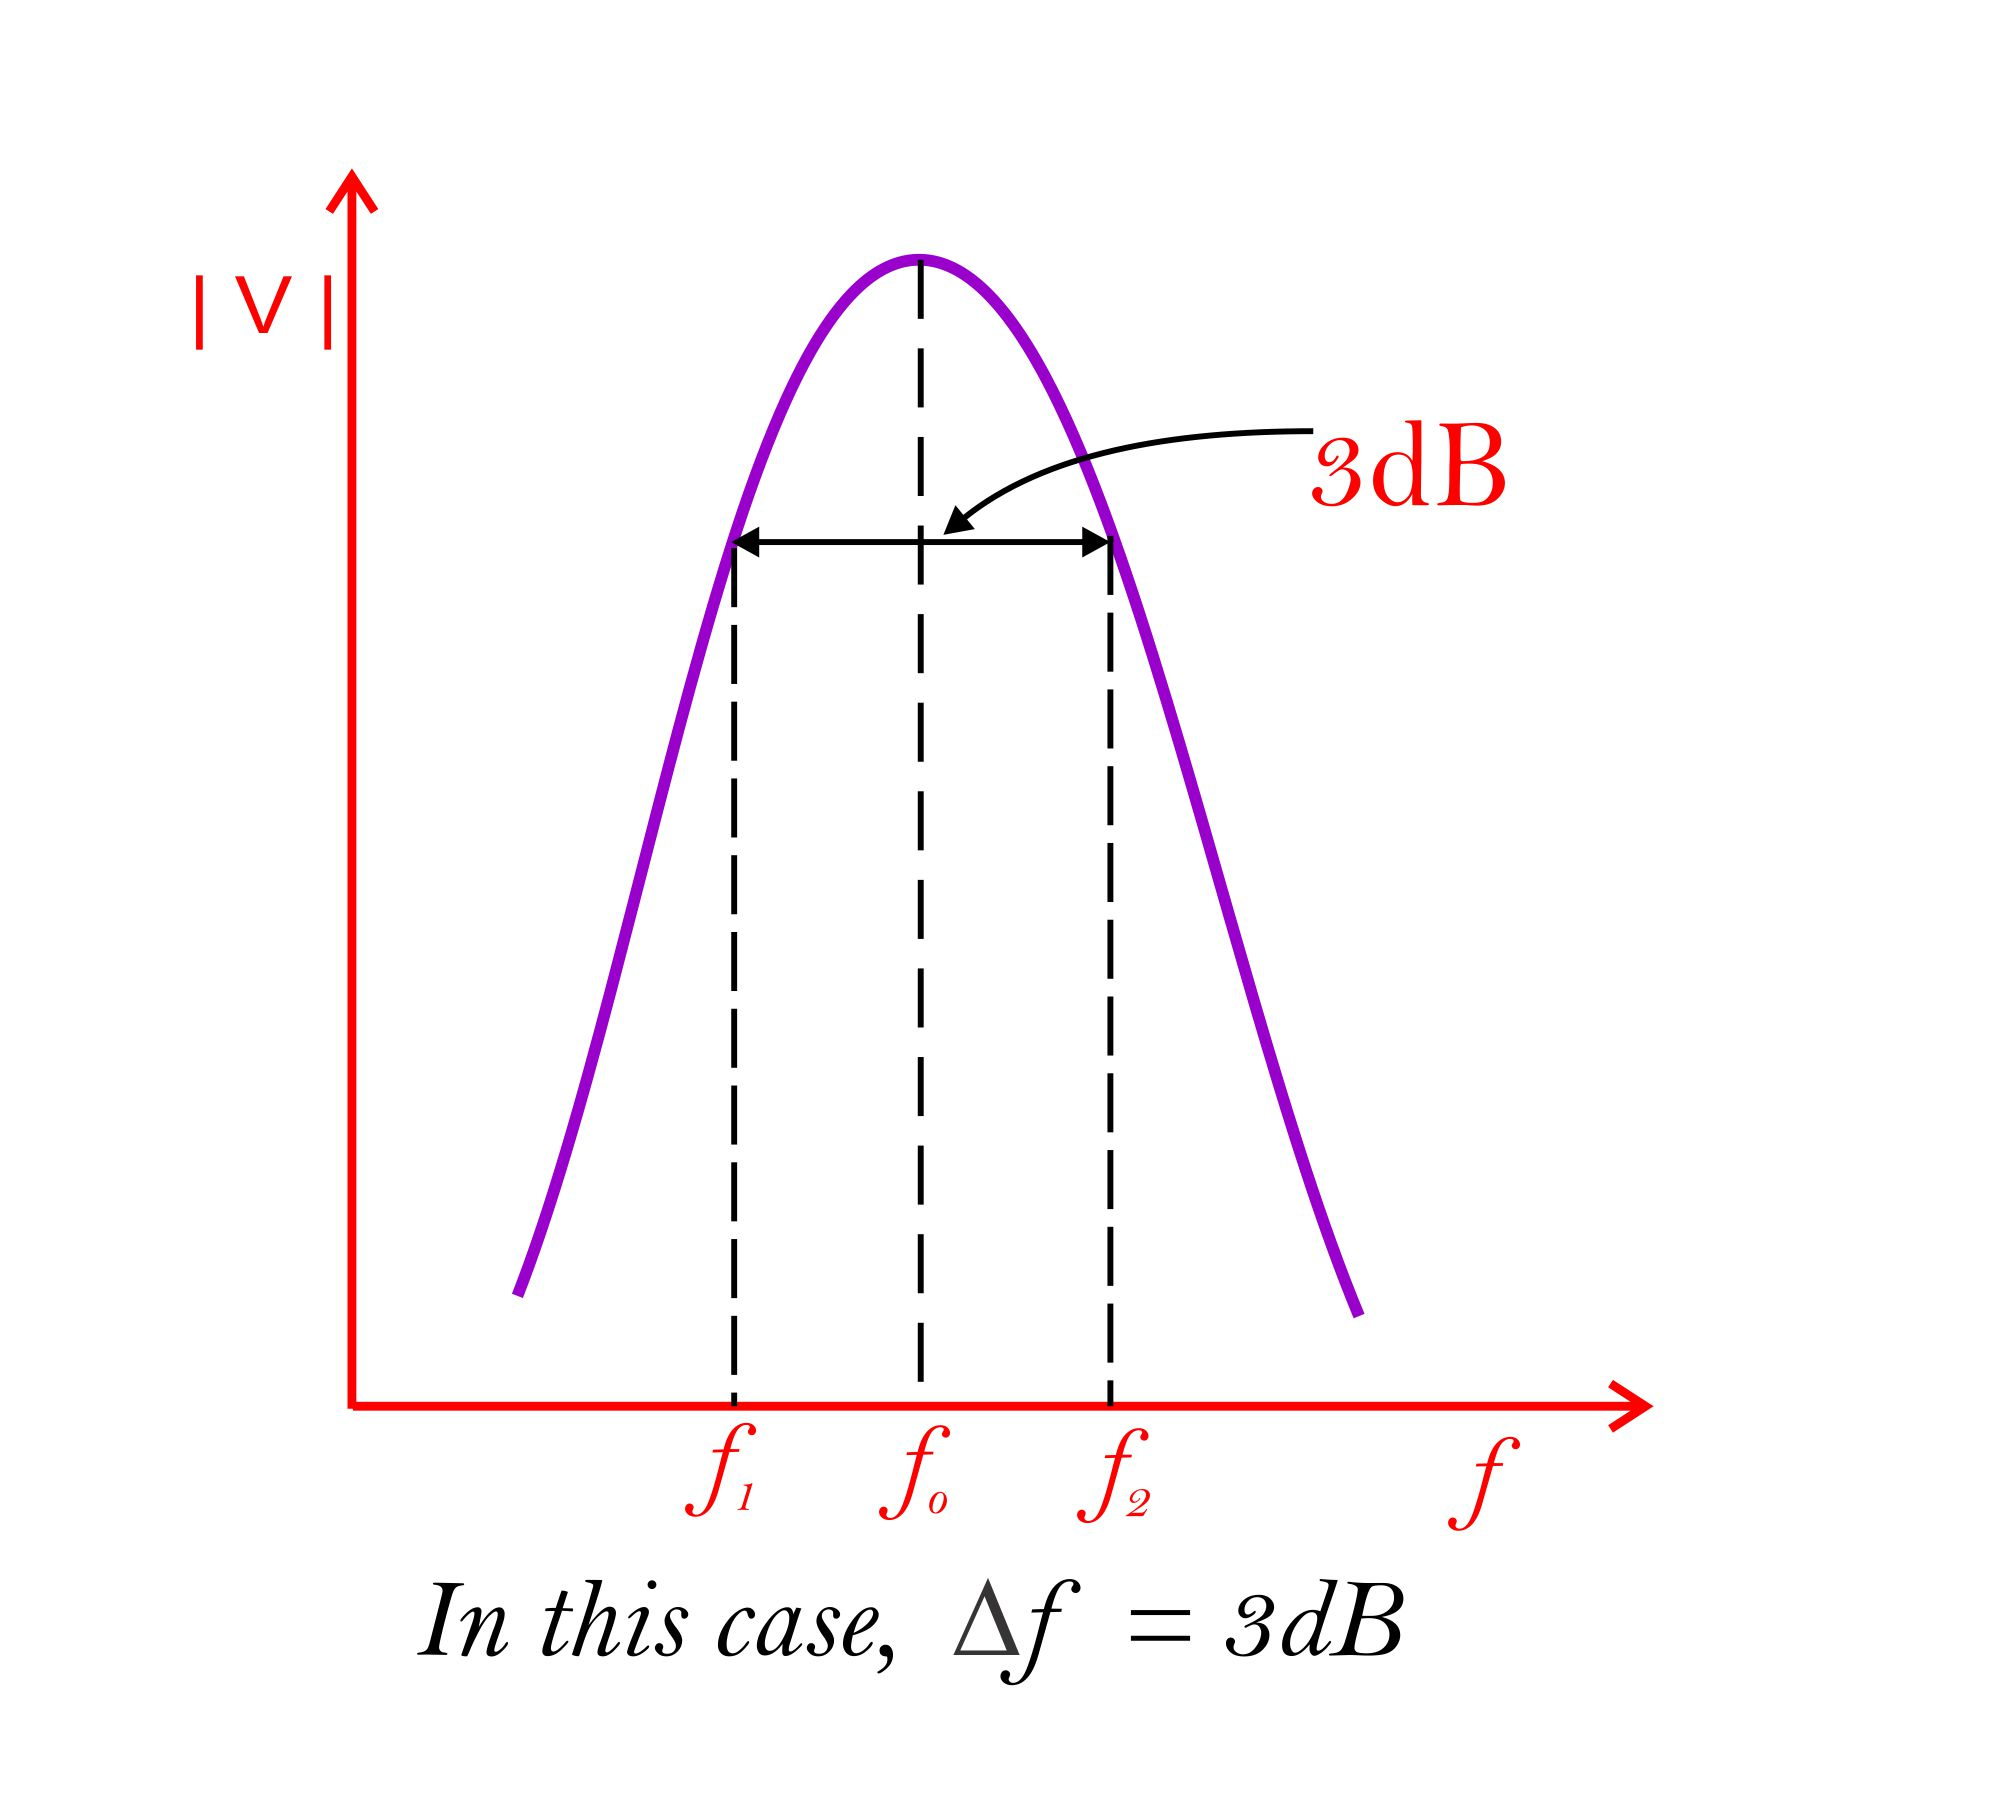
\includegraphics[width=0.8\linewidth]{\pathtopartone/graphics/fig2}
\caption{Frequency response of a resonant circuit}
\label{fig:fig2}
\end{figure}

The voltage response is shown in figure~\ref{fig:fig2}. It doesn't matter if we use a series or parallel resonance circuit. At resonance frequency $ f_0 $, we get the maximum response, below and beyond that frequency, the amplitude drops. The 3dB frequency is where the amplitude reduces to $ \frac{1}{\sqrt{2}} $ of its maximum value. In this case, $ \Delta f=3\text{dB bandwidth} =f_{2}-f_{1} $, so the quality factor is given as equation~\eqref{eqn:qualityfac}
\begin{equation}
Q=\frac{f_0}{\Delta f}=\frac{f_0}{f_{2}-f_{1}}
\label{eqn:qualityfac}
\end{equation} 

Alternatively, we can take a section of the transmission line, find the voltage distribution and current distribution in the transmission line, and then calculate the power loss. Then use this information to calculate the quality factor.
\begin{dmath*}
\text{Quality factor},Q 
=2\pi\left(\frac{\text{Energy stored in the circuit}}{\text{Energy lost per cycle}}\right) 
\end{dmath*} 
If the resonant frequency is $ f_0 $, the energy lost per cycle is $ f_0 $ cycles per second. Since in 1 second, we have $ f_0 $ number of cycles;
\begin{dmath*}
\text{Quality factor}, Q = 2\pi f_0\left(\frac{\text{Energy stored in the circuit}}{\text{Energy lost per second}}\right)
\end{dmath*}
The energy lost per second = Power loss in the circuit 
\begin{dmath*}
\text{Quality factor}, Q=2 \pi f_0\left(\frac{\text{Energy stored in the circuit}}{\text{Power loss in the circuit}}\right)
\end{dmath*}
So to calculate the quality factor, we calculate the energy stored in a section of the transmission line and the power loss in the transmission line. Then we can easily find out the value of the quality factor for that section of the transmission line.

let us consider a section of a short-circuited transmission line of length, $ l=\frac{\lambda}{4} $. Since the length depends on frequency, let us say frequency = $ f_0 $ when $ l=\frac{\lambda_{0}}{4}$ and carry out our analysis. Hence, the resonant frequency of a circuit is $ f_0 =\frac{v}{\lambda_{0}}$ (where $v$ = velocity of the wave). We now find voltage and current expression on the transmission line with the load end short-circuited. With the load end short-circuited, $Z_{L}= 0$, the reflection coefficient at the load point is -1 due to total reflection.

So,
\[\Gamma_{L} = \frac{Z_{L} - Z_0}{Z_{L} + Z_0} = \frac{0 - Z_0}{0 + Z_0} = -1\]
A reflection coefficient of -1 means that the amplitude of the reflection coefficient is 1 with a phase change of 180\textdegree.

At this point, we can write down the voltage and current equation with the known reflection coefficient. We can also find out what the variation of voltage and current is on the transmission line from equation~\eqref{eqn:voltagefromload}
\begin{dmath*}
V(l) = V^{+}e^{j\beta l} + V^{-}e^{-j\beta l},\quad \frac{V^{-}}{V^{+}}\text{ = } \Gamma, V^{-} \text{= }-V^{+}
= V^{+}e^{j\beta l} - V^{+}e^{-j\beta l}\text{Recall, }\frac{e^{j\beta l }- e^{-j\beta l}}{2j}\text{ = }\sin\beta l
=j2V^{+}\left(\frac{e^{j\beta l }- e^{-j\beta l}}{2j}\right) =j2V^{+}\sin \beta l\quad\text{Let, }j2V^{+}\text{ = }V_0
= V_0\sin \beta l 
\end{dmath*}
\begin{equation}
V(l) = V_0\sin \beta l
\label{eqn:voltagedistro}
\end{equation}
In a similar manner, we can find the current distribution using equation~\eqref{eqn:currentfromload},
\begin{dmath*}
I(l) = \frac{V^{+}}{Z_0}e^{j\beta l} - \frac{V^{-}}{Z_0}e^{-j\beta l},\quad\frac{V^{-}}{V^{+}}\text{ = }\Gamma, V^{-}\text{ = }-V^{+}
= \frac{V^{+}}{Z_0}e^{j\beta l} + \frac{V^{+}}{Z_0}e^{-j\beta l}\quad\text{Recall, }\frac{e^{j\beta l} + e^{-j\beta l}}{2}\text{ = }\cos \beta l
=\frac{2V^{+}}{Z_0}\left(\frac{e^{j\beta l} + e^{-j\beta l}}{2}\right)
= \frac{2V^{+}}{Z_0}\cos \beta l\quad\text{Let, }2V^{+}\text{ = }V_0
\end{dmath*}
\begin{equation}
I(l) = \frac{V_0}{Z_0}\cos \beta l
\label{eqn:currentdistro}
\end{equation}
\begin{figure}[h]
\centering
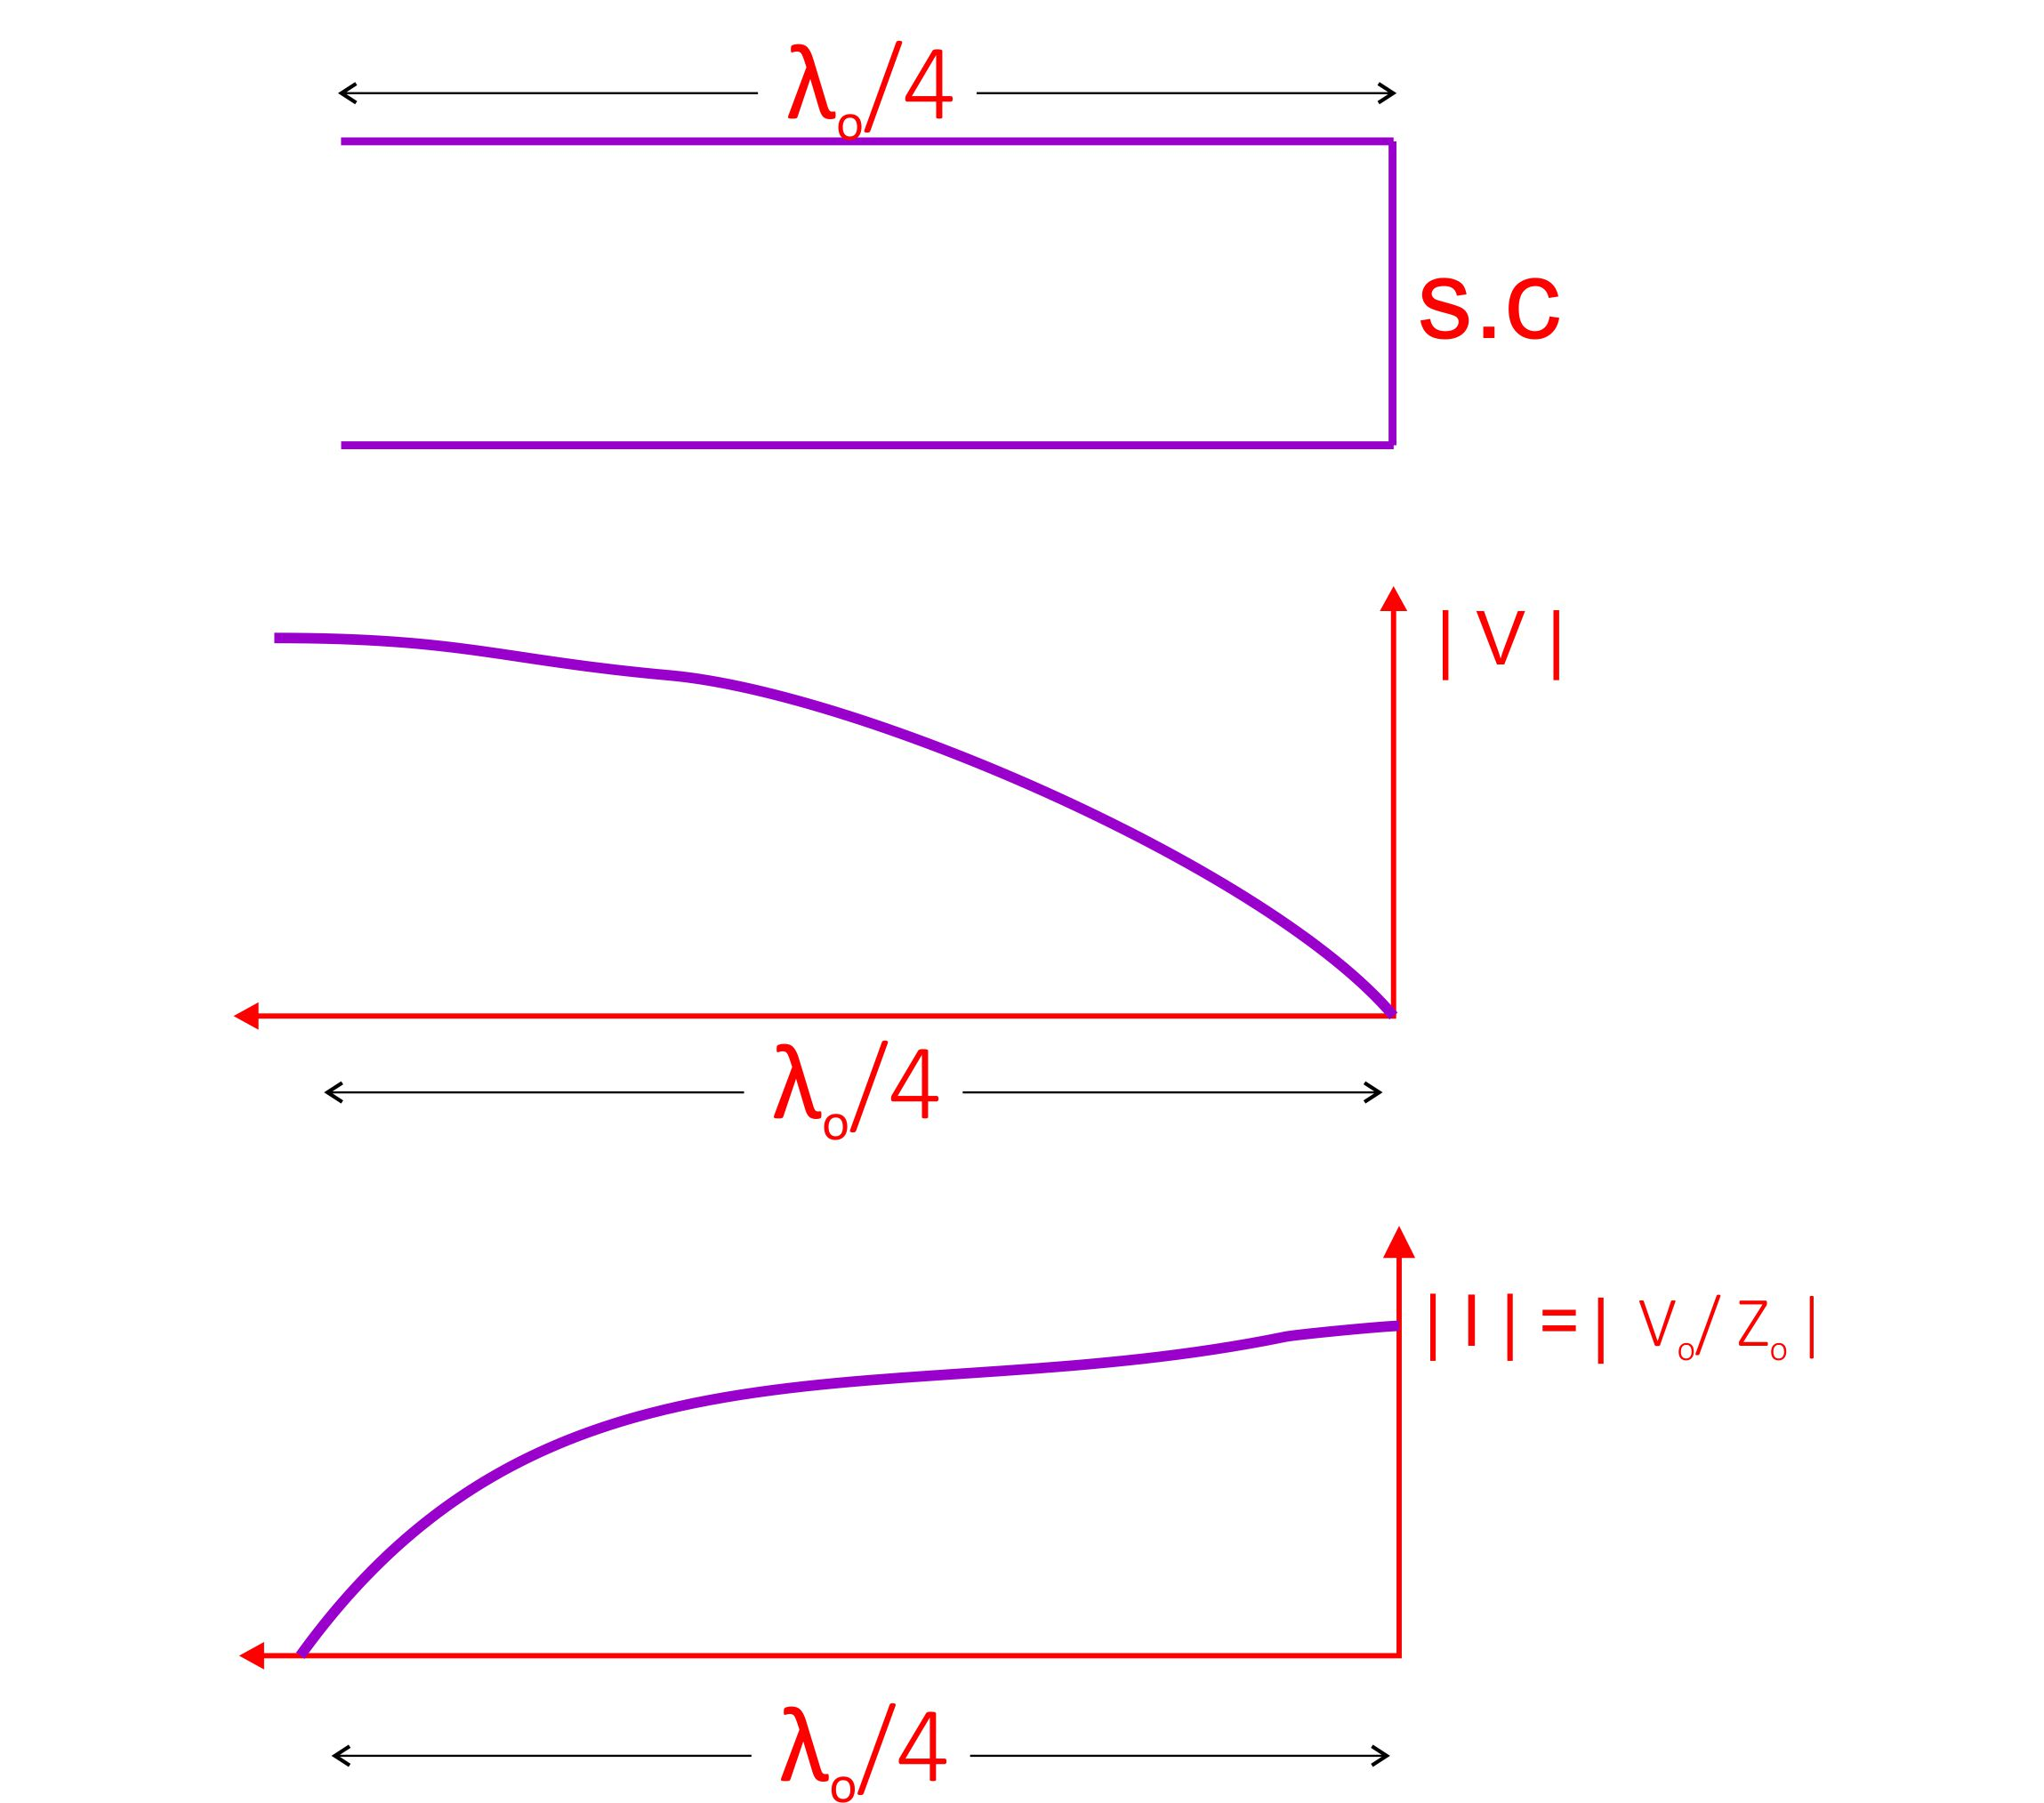
\includegraphics[width=1\linewidth]{\pathtopartone/graphics/fig03}
\caption{Voltage and Current distribution of the short-circuited transmission line}
\label{fig:fig03}
\end{figure}

The plot of the voltage and current distributions along the short-circuited transmission line is shown in figure~\ref{fig:fig03}. It is shown that at $l = \frac{\lambda}{2}$ the voltage distribution is maximum while that of the current is zero. At $ l = \frac{\lambda}{4}$ , $ \beta l = \frac{\pi}{2} $, so that $\sin \beta l = \sin \frac{\pi}{2}$ = 1 and $\cos \beta l = \cos \frac{\pi}{2} = 0$. For the voltage distribution, we have a peak at $ l = \frac{\lambda}{4}$ and a minimum of $ l = 0 $ and for the current distribution we have a peak value at $ l = 0$ and a minimum value at $l = \frac{\lambda}{4}$.

Now we know the voltage and current distributions on the section of the transmission line, we can find the energy stored at different points of the transmission line. To find the energy stored, the capacitance of an infinitesimal section of the transmission line is $C\Delta l$ for $\Delta l$ section since R, G, C and L are always stated per unit length. Hence, the capacitive and inductive energy stored in that section are 
\begin{align*}
U_{\text{capacitor}} = \frac{1}{2}C\Delta lV^{2}\\
U_{\text{inductor}} = \frac{1}{2}L\Delta lI^{2}
\end{align*}
Hence, the total energy stored in a transmission line can be written as:
\begin{dmath*}
U = \frac{1}{2}C\int_{0}^{\frac{\lambda_{0}}{4}}|V(l)|^{2}dl + \frac{1}{2}L\int_{0}^{\frac{\lambda_{0}}{4}}|I(l)|^{2}dl\quad\text{from equations~\eqref{eqn:voltagedistro} and~\eqref{eqn:currentdistro}}
= \frac{1}{2}C\int_{0}^{\frac{\lambda_{0}}{4}}|V_0\sin \beta l |^{2}dl + \frac{1}{2}L\int_{0}^{\frac{\lambda_{0}}{4}}\left|\frac{V_0}{Z_0}\cos \beta l \right|^{2}dl
= \frac{1}{2}CV_0^{2}\int_{0}^{\frac{\lambda_{0}}{4}}(\sin^{2} \beta l) dl + \frac{1}{2}L\frac{V_0^{2}}{Z_0^{2}}\int_{0}^{\frac{\lambda_{0}}{4}}( \cos^{2} \beta l) dl
\end{dmath*}
Recall from trigonometry   
\[\sin^{2} \beta l = \frac{1 - \cos2\beta l}{2},\quad \cos^{2} \beta l = \frac{1 + \cos2\beta l}{2}\]
{\small \begin{dmath}
U = \frac{1}{2}CV_0^{2}\int_{0}^{\frac{\lambda_{0}}{4}}\left(\frac{1}{2} - \frac{\cos 2\beta l}{2}\right) dl + \frac{1}{2}L\frac{V_0^{2}}{Z_0^{2}}\int_{0}^{\frac{\lambda_{0}}{4}} \left(\frac{1}{2} + \frac{\cos 2\beta l}{2}\right) dl  = \frac{1}{2}CV_0^{2}\left[\frac{l}{2} - \frac{\sin 2\beta l}{4 \beta}\right]_{0}^{\frac{\lambda_{0}}{4}} + \frac{1}{2}L\frac{V_0^{2}}{Z_0^{2}}\left[\frac{l}{2} + \frac{\sin 2\beta l}{4 \beta}\right]_{0}^{\frac{\lambda_{0}}{4}} = \frac{1}{2}CV_0^{2}\left[\frac{\lambda_{0}}{8} - \sin \frac{2(\frac{2\pi}{\lambda_{0}})\frac{\lambda_{0}}{4} }{4 \beta}\right] + \frac{1}{2}L\frac{V_0^{2}}{Z_0^{2}}\left[\frac{\lambda_{0}}{8} + \frac{\sin 2(\frac{2\pi}{\lambda_{0}})\frac{\lambda_{0}}{4} }{4 \beta}\right]= \frac{1}{2}CV_0^{2}\left[\frac{\lambda_{0}}{8} - \frac{\sin \pi}{4 \beta}\right] + \frac{1}{2}L\frac{V_0^{2}}{Z_0^{2}}\left[\frac{\lambda_{0}}{8} + \frac{\sin \pi}{4 \beta}\right] = \frac{1}{2}CV_0^{2}\left[\frac{\lambda_{0}}{8}\right] + \frac{1}{2}L\frac{V_0^{2}}{Z_0^{2}}\left[ \frac{\lambda_{0}}{8} \right]
\end{dmath}}
Where $\frac{1}{2}CV_0^{2}\left[\frac{\lambda_{0}}{8}\right] $ is the energy stored in line capacitance and $ \frac{1}{2}L\frac{V_0^{2}}{Z_0^{2}}\left[ \frac{\lambda_{0}}{8} \right] $ is the energy stored in line inductance.

We see that the two quantities are equal since
\begin{equation*}
Z_0 = \sqrt{\frac{L}{C}}\Longrightarrow CZ_0^{2} = L,\quad C = \frac{L}{Z_0^{2}}
\end{equation*}
\begin{dmath}
U = \frac{1}{2}CV_0^{2}\left[\frac{\lambda_{0}}{8}\right] +\frac{1}{2}CV_0^{2}\left[\frac{\lambda_{0}}{8}\right]
= \frac{1}{2}CV_0^{2}\left[\frac{\lambda_{0}}{4}\right]
\label{eqn:totalenergy}
\end{dmath}

Equation~\eqref{eqn:totalenergy} is the total energy in the short-circuited transmission line of length $l = \frac{\lambda_o}{4}$. To calculate the quality factor, we also need to calculate the power loss in the transmission line. If we take the section of a transmission line $\frac{\lambda_{0}}{4}$ shown in figure~\ref{fig:fig4}.
\begin{figure}[h]
\centering
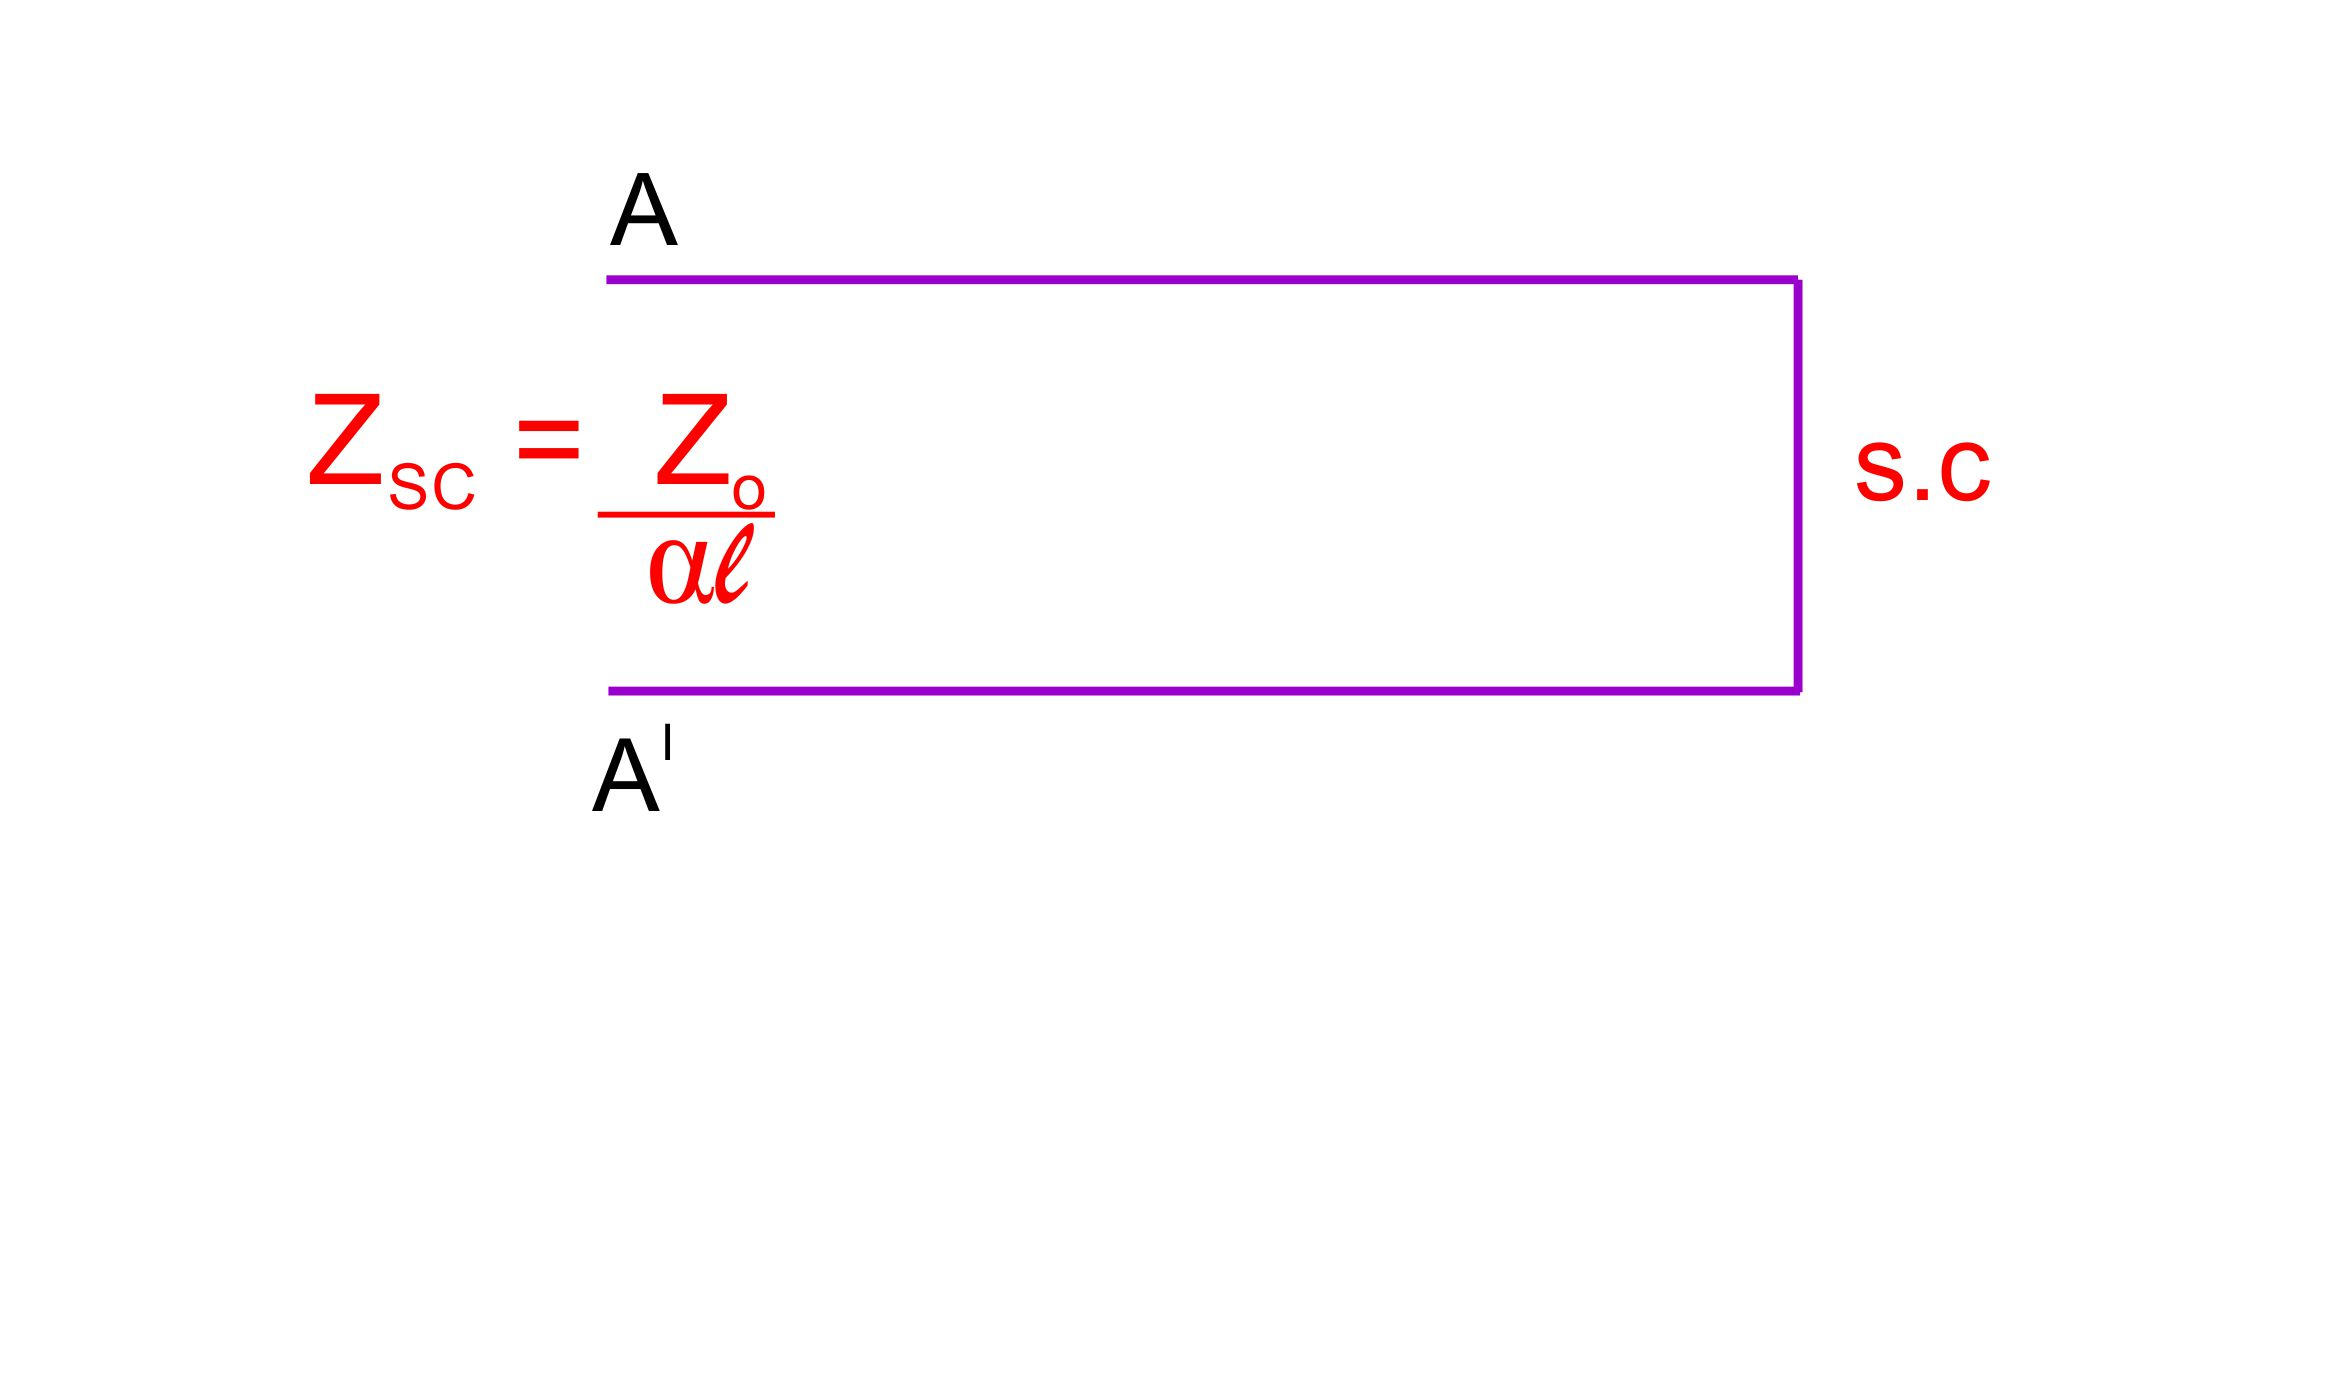
\includegraphics[width=1\linewidth]{\pathtopartone/graphics/fig4}
\caption{Input impedance of a short-circuited transmission line}
\label{fig:fig4}
\end{figure}

The energy stored in the line is connected at point AA'. Finding out what the power loss at AA' is, the power loss is equivalent to the power loss in the line because the line is short-circuited. Therefore, the load is not consuming any power and the power supplied will be equal to the loss in the transmission line. So without revisiting the primary constant of the transmission line, just by calculating the input impedance of the line, we can find out what the equivalent resistance would be at the input point of the line and find out the losses through this resistance which will be the power loss in the line. Hence, the input impedance seen at AA' will be
\begin{equation*}
Z_{SC} = \frac{Z_0}{\alpha l}\quad\text{from equation~\eqref{eqn:scimp}}
\end{equation*}
And the power loss is
\begin{dmath}
P_{loss} = \frac{V_0^{2}}{Z_{SC}}\quad V_0\text{ is the supplied voltage}
= \frac{V_0^{2}}{\frac{Z_0}{\alpha l}}
= \frac{\alpha l\times V_0^2}{Z_0}
= \frac{V_0^{2}}{Z_0}\times\alpha \times\frac{\lambda_{0}}{4}
\label{eqn:powerloss}
\end{dmath}
Then, the quality factor, Q from equation~\eqref{eqn:qualityfac} is given as follows by substituting equations~\eqref{eqn:totalenergy} and~\eqref{eqn:powerloss}.
\begin{dmath*}
Q = 2 \pi f_0\left(\frac{\frac{1}{2}\times CV_0^{2}\times\frac{\lambda_{0}}{4}}{\frac{V_0^{2}}{Z_0}\times\alpha \times\frac{\lambda_{0}}{4}}\right)
= 2 \pi f_0\left(\frac{\frac{1}{2}C}{\frac{\alpha}{Z_0}}\right)
= \frac{2 \pi f_0 Z_0C}{2\alpha}\quad\text{But, }Z_0\text{ = }\sqrt{\frac{L}{C}}\Rightarrow Z_0C\text{ = }\sqrt{LC}, 2\pi f_0\text{ = }\omega_{0}
= \frac{\omega_{0}\sqrt{LC}}{2 \alpha}\quad\omega_{0}\sqrt{LC}\text{ = }\beta\text{, phase constant}
= \frac{\beta}{2 \alpha}
\end{dmath*}
\begin{equation}
Q = \frac{\beta}{2 \alpha}
\label{eqn:qualityfacsoln}
\end{equation}
Equation~\eqref{eqn:qualityfacsoln} is the same expression we would have obtained by finding out the frequency response of the transmission line and measuring the input and its variation as a function of frequency. It implies that the quality factor is related to the phase $\beta$ and attenuation constant $ \alpha$ of the transmission line. For a low loss line $ \alpha \ll \beta$, thus Q is very large. This means that $Q \gg 1$ is for a low loss line. This is very important because it implies that at high frequencies, a section of a transmission line can give a high-quality factor circuit. Since the quality factor is related to 3dB bandwidth, the higher the quality factor, the smaller the 3dB bandwidth or the more tuned the circuit is. This is the frequency selectivity\index{frequency selectivity} of the circuit and a high-quality factor signifies a very frequency-selective circuit. We can get a few hundred to a few thousand quality factor values for some low-loss transmission lines and a very good frequency sensitivity section of a transmission line is used as a resonant circuit.

\subsection{As a Step Up Transformer}
Let us consider a small section of transmission line of length, $l = \frac{\lambda}{4}$, shorted at the end shown in figure~\ref{fig:fig5}. Let's say by some means, voltage is induced along the section of the transmission line not from open circuit or short circuit end but between these two ends which we will take as the middle location as shown by the dotted lines.
\begin{figure}[h]
\centering
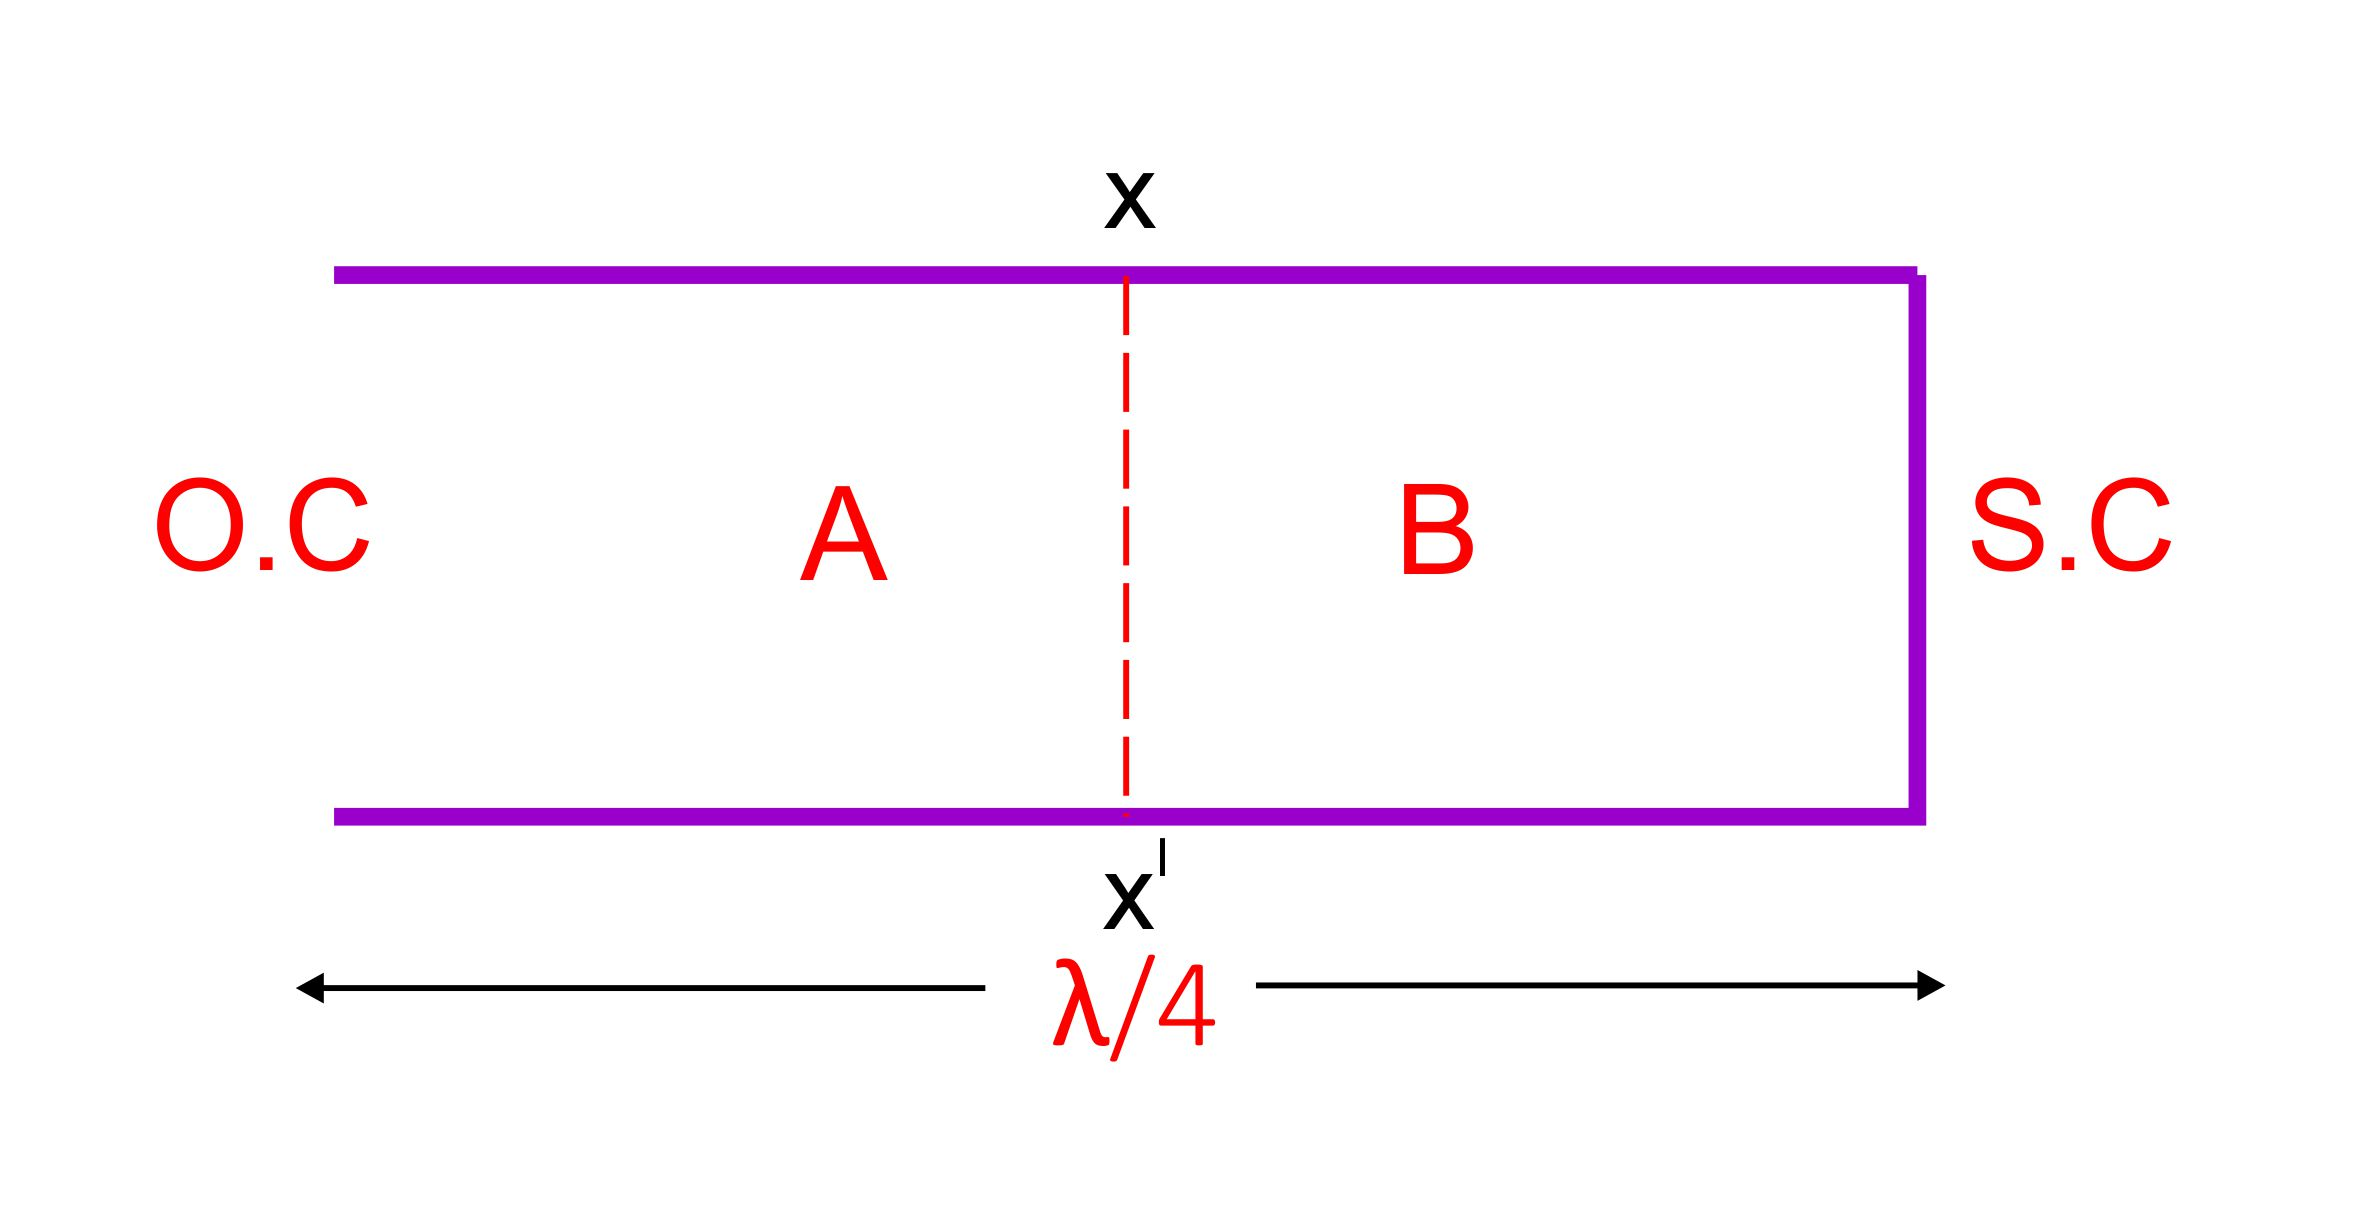
\includegraphics[width=1\linewidth]{\pathtopartone/graphics/fig5}
\caption{Voltage induced at the centre XX' of a transmission line of length $\frac{\lambda}{4}$ with one end open and the other end shorted}
\label{fig:fig5}
\end{figure}

 At any time, it would appear that the two sections, A and B, of the transmission line are connected in parallel. With the induced voltage, a standing wave signal will get induced in the transmission line. This standing wave (voltage and current distribution) does not see any impedance but the characteristic impedance of the transmission line. So the voltage at the middle point XX' sends two travelling waves along the transmission line as if the energy is supplied to the characteristic impedance of the two sections of the transmission line. The waves as shown in figure~\ref{fig:fig6} are going in directions M and N respectively.
 \begin{figure}[h]
\centering
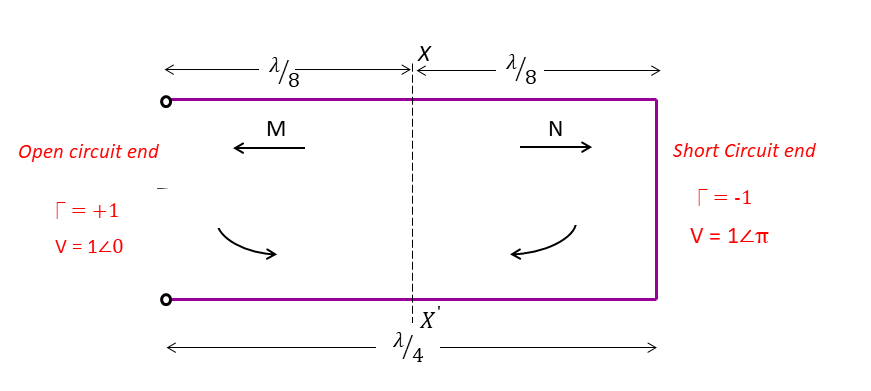
\includegraphics[width=1\linewidth]{\pathtopartone/graphics/step_up_transformer_application}
\caption{Standing wave propagation in the transmission line with one end open and the other end shorted}
\label{fig:fig6}
\end{figure}

 N travelling wave sees a short circuit and M travelling wave sees an open circuit. N wave sees a reflection coefficient of -1, hence, at the short circuit point, the wave is reflected completely as shown by the arrow. With a reflection coefficient of -1, the amplitude is unity but the phase is 180\textdegree (or $\pi$). Hence, the wave travelling toward N after reflection undergoes a phase change of $\pi$ and travels all the way to the open circuit side. At the open circuit point, the reflection coefficient = 1\footnote{
\begin{dmath*}
\Gamma_{L} = \frac{Z_{L} - Z_0}{Z_{L} + Z_0}\quad Z_{L}\text{ = }\infty\text{ and taking limits}
= \frac{1 - \frac{Z_0}{Z_{L}}}{1 + \frac{Z_0}{Z_{L}}}
= \frac{1 - \frac{Z_0}\infty}{1 + \frac{Z_0}\infty}
= \frac{1 - 0}{1 + 0}
= 1
\end{dmath*}
}. The reflected N wave reverses with $\pi$ phase change gets to an open circuit with a reflection coefficient of 1, turns around and moves to point XX'. The distance traveled by the wave is $ \frac{\lambda}{2} = \frac{\lambda}{8} + \frac{\lambda}{4} + \frac{\lambda}{8}$ and has gone through a phase change of $2\pi$. This is because a travel distance of $\frac{\lambda}{4}$ corresponds to a phase change of $\pi$ plus another $\pi$ phase change due to a negative reflection coefficient. It means N wave has undergone a phase change of $\pi$ due to $\frac{\lambda }{4}$ distance travelled + $\pi$ due to the negative reflection coefficient at the short circuit end, resulting in a total phase change of $2\pi$. Hence the wave that is induced at XX' is the same as the wave N which has been taken through a phase change of $2\pi$. This is some kind of positive feedback because the induced voltage will add to the reflected voltage N, increase in amplitude and then the resulting constructive interference re-travels and repeats. That means the voltage essentially starts growing in the transmission line.

Exactly the same thing happens to the travelling wave M. It will be reflected at the open circuit end, travel $\frac{\lambda}{4}$ to the short circuit end, reverse with a phase of $\pi$ and travels towards XX'. At the end has travelled $\frac{\lambda }{2}$ distance with a total phase change of $2\pi$. Thus at point XX' the returned wave adds to the induced voltage at XX'. Then the resulting voltage at XX' grows as the travelling waves travel a trip one more time. Hence the standing wave of the setup will grow.

Now we ask the question, \emph{how far will an induced voltage at XX' grow?} With no losses in the transmission line, it will grow up to infinity. The voltage will keep growing to infinite amplitude because there is nothing controlling this amplitude on the transmission line. Hence, if even a small voltage is induced on a section of the transmission line with resonant length, the resulting standing wave in the transmission line is much larger compared to the induced voltage on the transmission line. This resonant section of the transmission line can then be used as a voltage step-up transformer. Hence, we would measure a much larger voltage at the open section of the line i.e. at an open circuit compared to what we induced at point XX'. In theory, with no losses in the transmission line, this voltage amplitude should grow to infinity. However, that does not happen because as voltage and current amplitude is increasing in the transmission line, the ohmic losses also are increasing. When the losses in the line due to resistance and conductance (R and G) become equal to the energy source, at that point there is energy balance and the growth of the standing wave in the section of the transmission line stops.

Its application as a step-up transformer involves the connection of a small coupling source to generate a very large voltage and current when the losses are small. This is a useful application whenever we want to step up a voltage or current at high frequencies. It can be shown that this voltage growth is related to the quality factor of a transmission line. The higher the quality factor, the lower the losses in the transmission line and that will give higher voltages on the terminal of the transmission line.

The phenomena used here for voltage step-up could be harmful in many cases. Consider a situation where a small energy source gets unknowingly coupled to a small section of the transmission line. If the section of the transmission line is of resonance length, then the voltage developed on this line will be much larger than the circuit can handle and this can damage the circuit. Thus while designing high-frequency circuits, we should be careful not to couple some sections to the transmission line especially if they are of resonant length, otherwise, we develop a large voltage in that section that the circuit can barely handle. 

With the applications of transmission lines we have discussed so far when sections of transmission lines are used for high-frequency circuits, we rarely see capacitors and inductors because they have been replaced by sections of transmission lines. What we see instead are active devices like transistors and FETs with reactive components completely realized by sections of the transmission line. So most microwave circuits will appear as transmission lines across active devices.

\section*{Exercises}
\begin{ExerciseList}
\Exercise[label={ex111}]
A transmission line of length $\frac{\lambda}{4}$ is shorted at one end and open at the other end. If a voltage of 1V is induced at the centre of the transmission line, what is the voltage at the open circuit end?
\Answer
Solution to exercise~\ref{ex111}
\end{ExerciseList}
